\documentclass[11pt, a4paper, spanish, openright, twoside]{book}
\usepackage[spanish, activeacute]{babel}
\usepackage[utf8]{inputenc}
%\usepackage[top=2.5cm, bottom=2.5cm, outer=1.75cm, inner=1.75cm, heightrounded, marginparwidth=2.5cm, marginparsep=0.3cm]{geometry}	%márgenes empequeñecidos
\usepackage[top=2.95cm, bottom=2.25cm, outer=2.75cm, inner=2.75cm, heightrounded, marginparwidth=2.5cm, marginparsep=0.3cm]{geometry}	%márgenes originalmente
\usepackage{dpg}
\usepackage{fli}

\usepackage{pgf}
\usepackage{tikz}

\usepgflibrary{shapes.geometric} % LATEX and plain TEX and pure pgf
\usetikzlibrary{arrows,automata,positioning}
\tikzstyle{accepting by double}= [double distance=1.6pt,double,outer sep=.5\pgflinewidth+.8pt] % esto es algo estético.
\renewcommand\shorthandsspanish{}  % para compatibilizar spanish con tikz

%%%%%%		Figuras		%%%%%%%%%%%%%%%%%%%
\usepackage[vflt]{floatflt}		%Entorno float-figure

%%%%%%		Page style		%%%%%%%%%%%%%%%%%%%
\renewcommand{\thepage}{\arabic{page}}% Arabic page numbers\fancyhead{}
\pagestyle{fancy}
\fancyfoot{}
\fancyhead[LO,RE]{Práctica 2}	%encabezado de pares: nombre de la sección
\fancyfoot[LE,RO]{\thepage}	%abajo a izqda en pares, derecha en impares: numero de pagina
%\fancyhead[LE]{\nouppercase{\leftmark}} %cuadro izquierdo de pagina par: parte y contador
\fancyfoot[CE]{Inteligencia Artificial} 
\fancyfoot[CO]{Doble Grado Informática-Matemáticas - Universidad Complutense}
\renewcommand{\footrulewidth}{0.4pt}
\renewcommand{\headrulewidth}{0.4pt}		% linea por debajo del encabezado
\renewcommand{\sectionmark}[1]{\markright{\textbf{\thesection. #1}}}	%negrita
\renewcommand{\labelitemi}{$\circ$} %Primer itemize con circunferencia vacia
\renewcommand{\labelitemii}{} %Segundo itemize con punto pequeño \cdot
\renewcommand*{\thesection}{\arabic{section}}	% Hace que no apareca el indice de capitulos y que comience en section

%%%%%%		Others		%%%%%%%%%%%%%%%%%%%
\setlength{\leftmarginii}{0em} %Segundo itemize sin sangria
\setlength{\leftmarginiii}{1em} %Tercer itemize casi sin sangria
\renewcommand{\labelitemiii}{ }
\pagenumbering{roman}
\addto{\captionsspanish}{\renewcommand*{\contentsname}{Índice}} %Cambia "Indice general" por "Indice"



\begin{document} 
\title{\Huge{\textsc{Inteligencia Artificial}} \\
	\vspace{0.7cm}
	 \textsc{\Large{Práctica 2}} \\
	\vspace{1.5cm}
	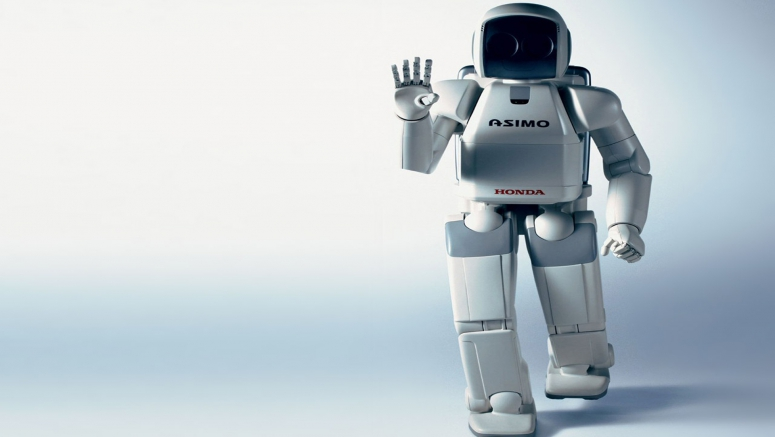
\includegraphics[scale=0.45]{robotHonda}}
\author{Enrique Ballesteros Horcajo\\
	Ignacio Iker Prado Rujas}
\date{\Today}
\maketitle

\newpage
\mbox{}
\thispagestyle{empty}						% Hoja en blanco, sin numeros ni nada
\newpage


\tableofcontents 							%INDICE hipervinculado

\newpage
\mbox{}
\thispagestyle{empty}						% Hoja en blanco, sin numeros ni nada
\newpage

\pagenumbering{arabic}						% Pone el contador de paginas a 1 y ahora en numeros normales

\vspace{3cm}


\newpage



\begin{section}{Introducción: AimaDemoApp}

Para esta primera parte, tras haber importado el proyecto a Eclipse, hemos ejecutado el fichero \texttt{AimaDemoApp.java}, probando las distintas posibilidades que ofrece. Tiene dos modos: \textit{Applications} y \textit{Demos}, y la principal diferencia está en que en la primera disponemos de una interfaz gráfica, útil para comprender mejor qué esta haciendo el algoritmo correspondiente. 

La primera aplicación que podemos usar es para el coloreado de mapas mediante \textit{backtracking} con distintas heurísticas. Es muy interesante ejecutar la aplicación paso a paso, para ver como se desarrolla el árbol. Además, hay algunos juegos como el puzzle de 8, el 3 en raya, las $n$-reinas y el conecta 4. Los algoritmos que utilizan son los habituales, con algunas variaciones en la heurística: minimax, poda $\alpha-\beta$, búsqueda en anchura, búsqueda en profundidad, $A^*$, voraz... Además, incluye una aplicación para encontrar el camino mínimo entre dos nodos de un grafo, que aquí es un mapa de Rumanía y otro de Australia. %Por ultimo, ni puta idea de que concha es la útlima app.

Luego, en cuanto a las demos, aparecen algunas aplicaciones nuevas, pero creemos que tiene menos interés porque sólo puedes ver el resultado final y tratar de interpretarlo, y no puedes modificar parámetros como en las aplicaciones anteriores, o incluso interferir en los juegos haciendo el movimiento que quieras. 

	\begin{table}	
		\begin{center}
			\begin{tabular}{|c||c|c|c|c|}
				\hline	Petaqueo	& \texttt{del} 	& \texttt{bueno} 	& \texttt{every} & \texttt{day}\\ \hline \hline
				\textbf{Vale} 	&  	4,8 ms	& 	2 ms	 & 	0,7 ms		& 6 ms	  \\ \hline 
				\textbf{Kike?}  	&  	3,5 ms	& 	2,7 ms	 & 	3 ms		& 5,8 ms	 \\ \hline 				
			\end{tabular}
		\caption{Esto es un guión de tabla.}
		\end{center}
	\end{table}

\end{section}

\begin{section}{Puzle de 8 extremo}

	
\end{section}

\begin{section}{AimaDemoApp: Desde Arad hasta Bucharest}


%3) Ejecuta AimaDemoApp en modo aplicación para la búsqueda de caminos en el mapa de Rumanía, desde Arad a Bucharest, utilizando la búsqueda en profundidad, en anchura y el algoritmo A* con la heurística de la distancia en línea recta. Haz una tabla con los resultados obtenidos con cada algoritmo e incorpórala a la memoria. Interpreta y discute los resultados. ¿Por qué el algoritmo de búsqueda en anchura no obtiene el camino mínimo?
	
SLD es la heurística de línea recta, que elige la ciudad que está más cerca en línea recta del objetivo. En el cuadro adjunto podemos ver como se desarrolla el algoritmo en cada caso. Cabe destacar también que en el primero se expanden 10 nodos, mientras que en el segundo y en el tercero son 5.

El algoritmo de la búsqueda en anchura no encuentra el camino mínimo porque %, ¿por qué Kike?

	\begin{table}	
		\begin{center}
			\begin{tabular}{|c||c|c|c|c|}
				\hline \textbf{Arad-Bucarest}	& \textbf{Depth First} 	& \textbf{Breadth First} 	& $A^*$ \\ \hline \hline
				\textbf{Step 1} 			&  	Timisoara - 118	& Sibiu - 140			& Sibiu - 140			\\ \hline 
				\textbf{Step 2} 			&  	Lugoj - 229		& Fagaras - 239		& RimnicuVilcea - 220	\\ \hline 
				\textbf{Step 3} 			&  	Mehadia - 299		& Bucarest - 450		& Pitesti - 317			\\ \hline 
				\textbf{Step 4} 			&  	Dobreta - 374		& -					& Bucarest - 418		\\ \hline 
				\textbf{Step 5} 			&  	Craiova - 494		& -					& -					\\ \hline 
				\textbf{Step 6} 			&  	Pitesti - 632		& -					& - 					\\ \hline 
				\textbf{Step 7} 			&  	Bucharest - 733	& -					& -					\\ \hline \hline
				\textbf{Total} 			&  	733 in 7 steps		&  450 in 3 steps		& 418 in 4 steps		\\ \hline 

			\end{tabular}
		\caption{Para la búsqueda de caminos en el mapa desde Arad hasta Bucarest, comparación entre la búsqueda en profundidad, en anchura y el $A^*$ con SLD.}
		\end{center}
	\end{table}


\end{section}


\begin{section}{SearchDemoOsmAgentApp: Desde Altheim hasta Leibi}


\end{section}


\begin{section}{Librerías y definiciones de estado para el puzzle de 8 }

Para el problema del puzle de 8 se utiliza un array de enteros de tamaño 9, sencillo pero efectivo. El rango de valores para el vector es $0\le i \le 8$ (sin repeticiones), y de este modo el cero corresponde al hueco en el puzle. El resto de casillas se corresponden 1-1 con su representación gráfica, leído de izquierda a derecha y de arriba a abajo. Además, se define en \texttt{EightPuzzleBoard.java} en el paquete \texttt{aima.core.enviroment.eightpuzzle} como array privado de enteros. También es importante notar que en función de desde donde se llame al constructor de esta clase, se pasa como parámetro un vector diferente (en función de la dificultad). 

\begin{figure}[!h]
		\begin{center}
			%\hspace{-0.5cm}
			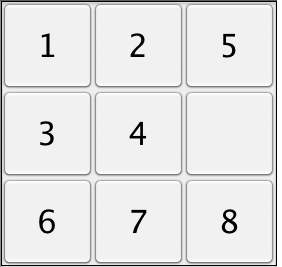
\includegraphics[scale=0.65]{puzle8}
			\caption{Puzle de 8 correspondiente a \texttt{state = new int$[] \{ 1, 2, 5, 3, 4, 0, 6, 7, 8 \}$}.}
		\end{center}
	\end{figure}
\end{section}

En cuanto a los operadores que trabajan con el estado, \textit{se centran en el hueco} y hay cuatro: \texttt{moveGapLeft()}, \texttt{moveGapUp()}, \texttt{moveGapRight()}, \texttt{moveGapDown()}. Hacen lo propio, tras comprobar que pueden hacer el movimiento pedido con \texttt{CanMoveGap()} calculan en qué posición está el hueco y cambian sus coordenadas en el mapa hacia la izquierda, arriba, derecha o abajo respectivamente. Para ello simplemente hacen un \textit{``swap''}, guardando (por ejemplo para el primer caso) el valor situado a la izquierda del cero, poniéndolo a la derecha y escribiendo un cero a la izquierda. Es interesante ver como transforman un tablero $3\times 3$ en un vector lineal de 9 posiciones. Dadas las coordenadas $(x,y)$ la posición correspondiente en el vector es $3x + y$ (contando como (1,1) la esquina inferior izquierda donde está el 6 en la imagen), y así por ejemplo, en la figura vemos que 7 está en las coordenadas $(2,1)\implies 3\cdot 2 + 1 = 7$, luego \texttt{state[7] = 7}. Esto se consigue mediante las funciones \texttt{getAbsPosition()} y \texttt{setValue()}, en la misma clase que la comentada anteriormente.

En el paquete \texttt{aima.core.environment.eightpuzzle} se encuentra la clase donde se calcula el número de fichas descolocadas: \texttt{MisplacedTilleHeuristicFunction.java}.



\begin{section}{Librerías y definiciones de estado para el mapa }


\end{section}

	
\section{Conclusiones}


	
\begin{thebibliography}{9}

\bibitem{aima}
	Russell, S.; Norvig, P, \\
	\emph{Artificial Intelligence, a modern aproach}.\\
	New Jersey: Pearson, 2010.
	
\bibitem{clase}
	Apuntes y transparencias de Inteligencia Artificial, \\
	Doble Grado Matemáticas - Ing. Informática, U.C.M., 2014-2015.

\end{thebibliography}


\end{document}

